\documentclass[12pt,aspectratio=169,english,finnish,pdflatex%,handout
]{beamer}
\definecolor{MyGreen}{RGB}{50, 120, 50}
\usecolortheme[named=MyGreen]{structure}
% \setbeameroption{show notes} 


\usepackage{babel}
\usepackage[utf8]{inputenc}
\usepackage[T1]{fontenc}
\usepackage{amsmath,amssymb} 
\usepackage{animate}
\usepackage{multimedia}

\usepackage{natbib}
\bibpunct[: ]{(}{)}{,}{}{}{;}

\usepackage{tikz}

\usepackage{tipa}

\usepackage{hyperref}

\setbeamertemplate{navigation symbols}{}

\graphicspath{{figures/}}

\setlength{\leftmargini}{0pt}
\setlength{\leftmarginii}{1em}

%% Write out the names of graphics files being included 
\newwrite\graphics
\immediate\openout\graphics=\jobname.graphics%
\let\oincludegraphics\includegraphics% store original \includegraphics
\renewcommand{\includegraphics}[2][]{% prepend to it (could also use xpatch, etc.)
  \immediate\write\graphics{#2}
  \oincludegraphics[#1]{#2}}

\newcommand{\kommentti}[1]{
  {\bf[#1]}
}


% \setbeamertemplate{title page}{
%   \vbox{}
%   \vfill
%   \begingroup
%     \centering
%     \usebeamertemplate{title}
%     \vskip0.5em
%     \usebeamertemplate{author}
%     \usebeamertemplate{date}
%     \vskip1em
%     \usebeamertemplate{titlegraphic}
%   \endgroup
%   \vfill
% }
\defbeamertemplate*{title page}{customized}[1][]
{
  \centering
  \usebeamerfont{title}{\usebeamercolor[fg]{subtitle}\inserttitle}\par
  \bigskip
  \usebeamerfont{subtitle}\usebeamercolor[fg]{black}\insertauthor\par
  \usebeamerfont{subtitle}\insertdate\par
  \bigskip
  % \inserttitlegraphic
}

\title{My three priorities for impact in\\
SLT/SLP research and teaching
}
\author{Pertti Palo, PhD, Lic. Tech., MSc} 
\date{5 May 2026} 

\begin{document}

\frame{\titlepage
  \centering
  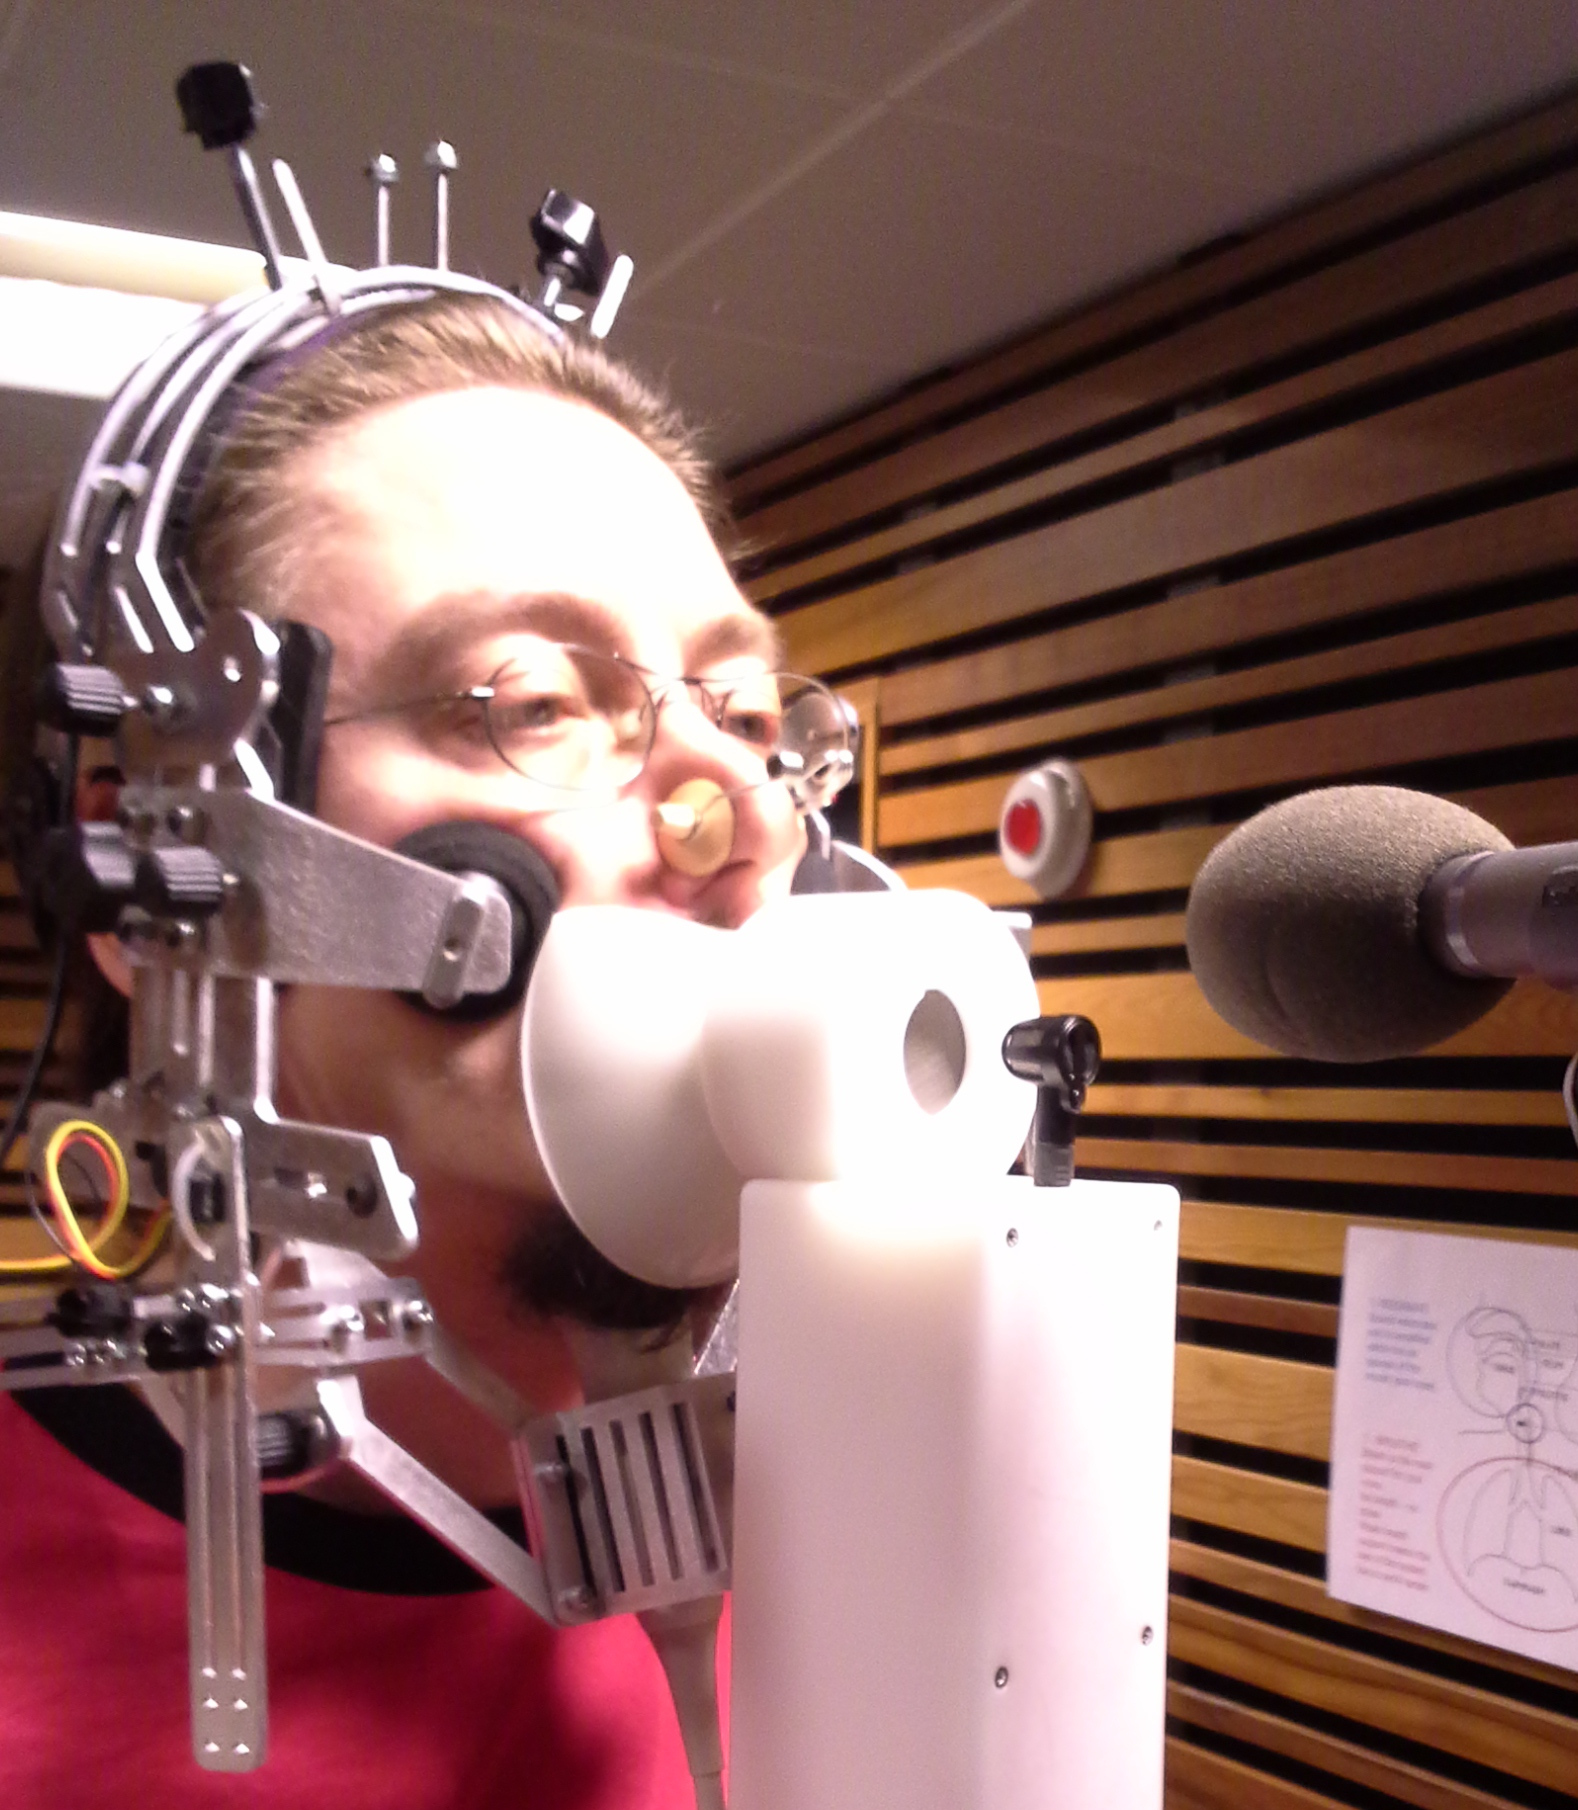
\includegraphics[height=3cm]{ultra-eva.jpg}
  % 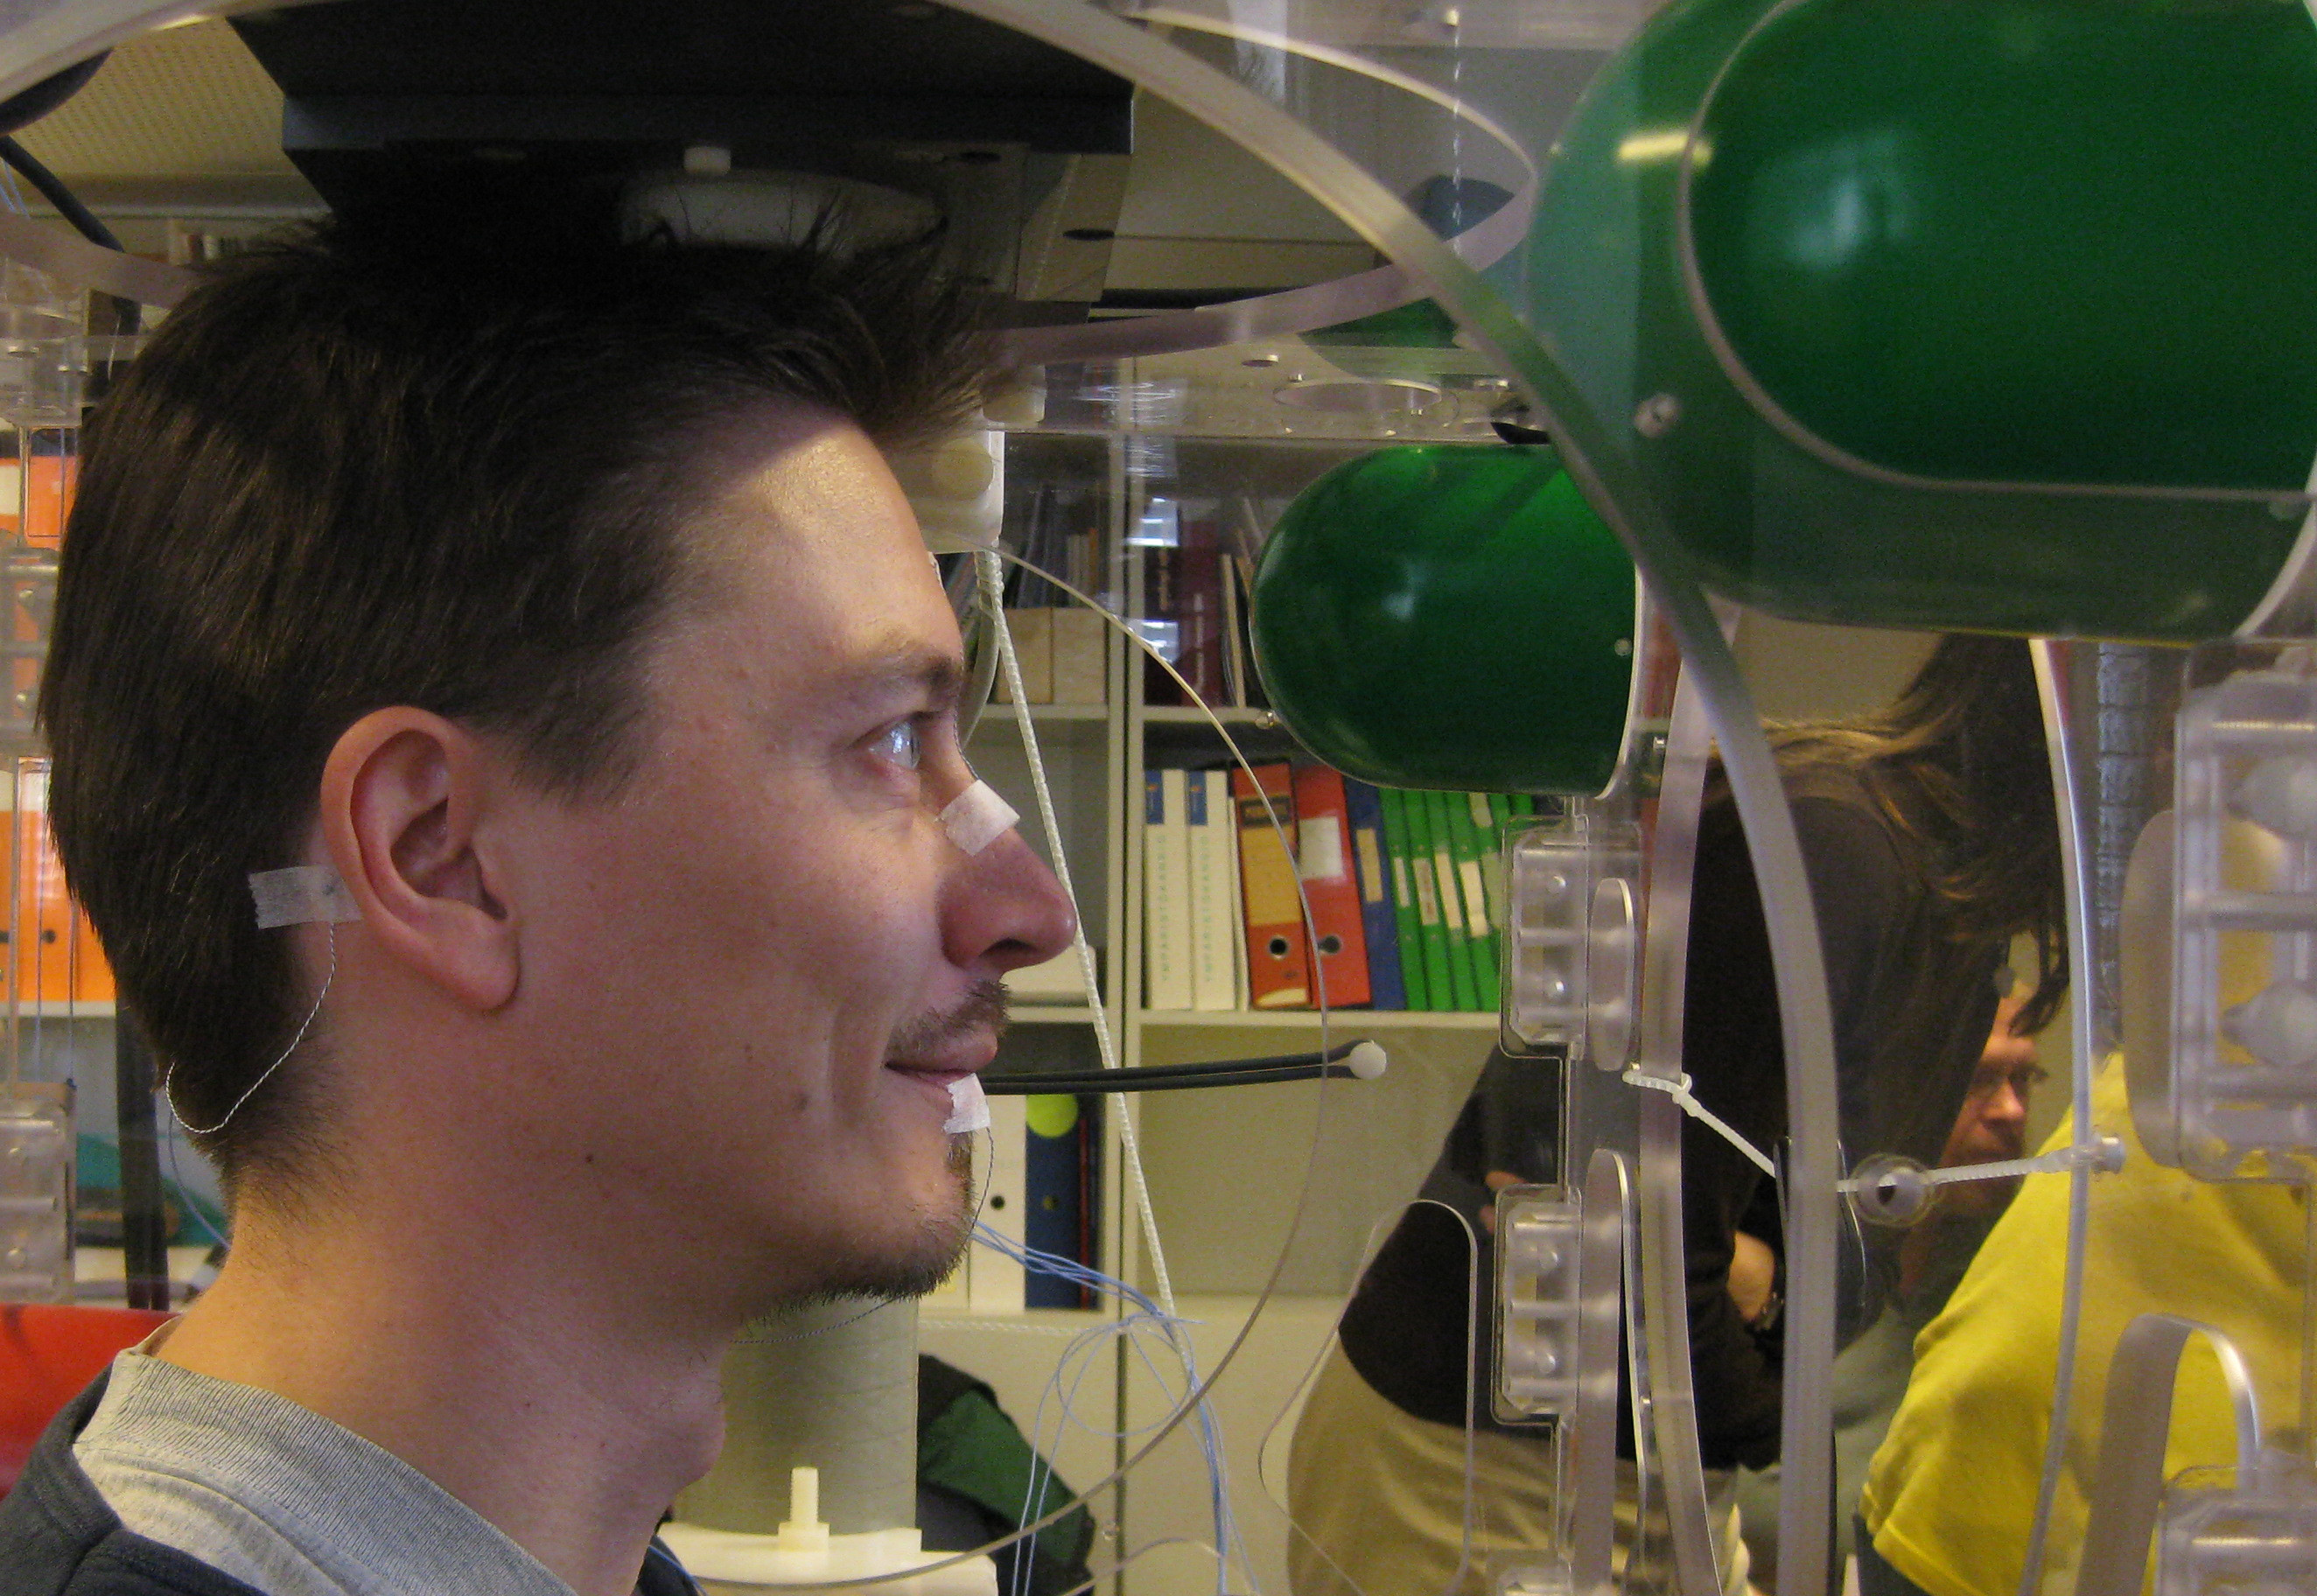
\includegraphics[height=3cm]{ema_kauan_sitten_cropped.JPG}
  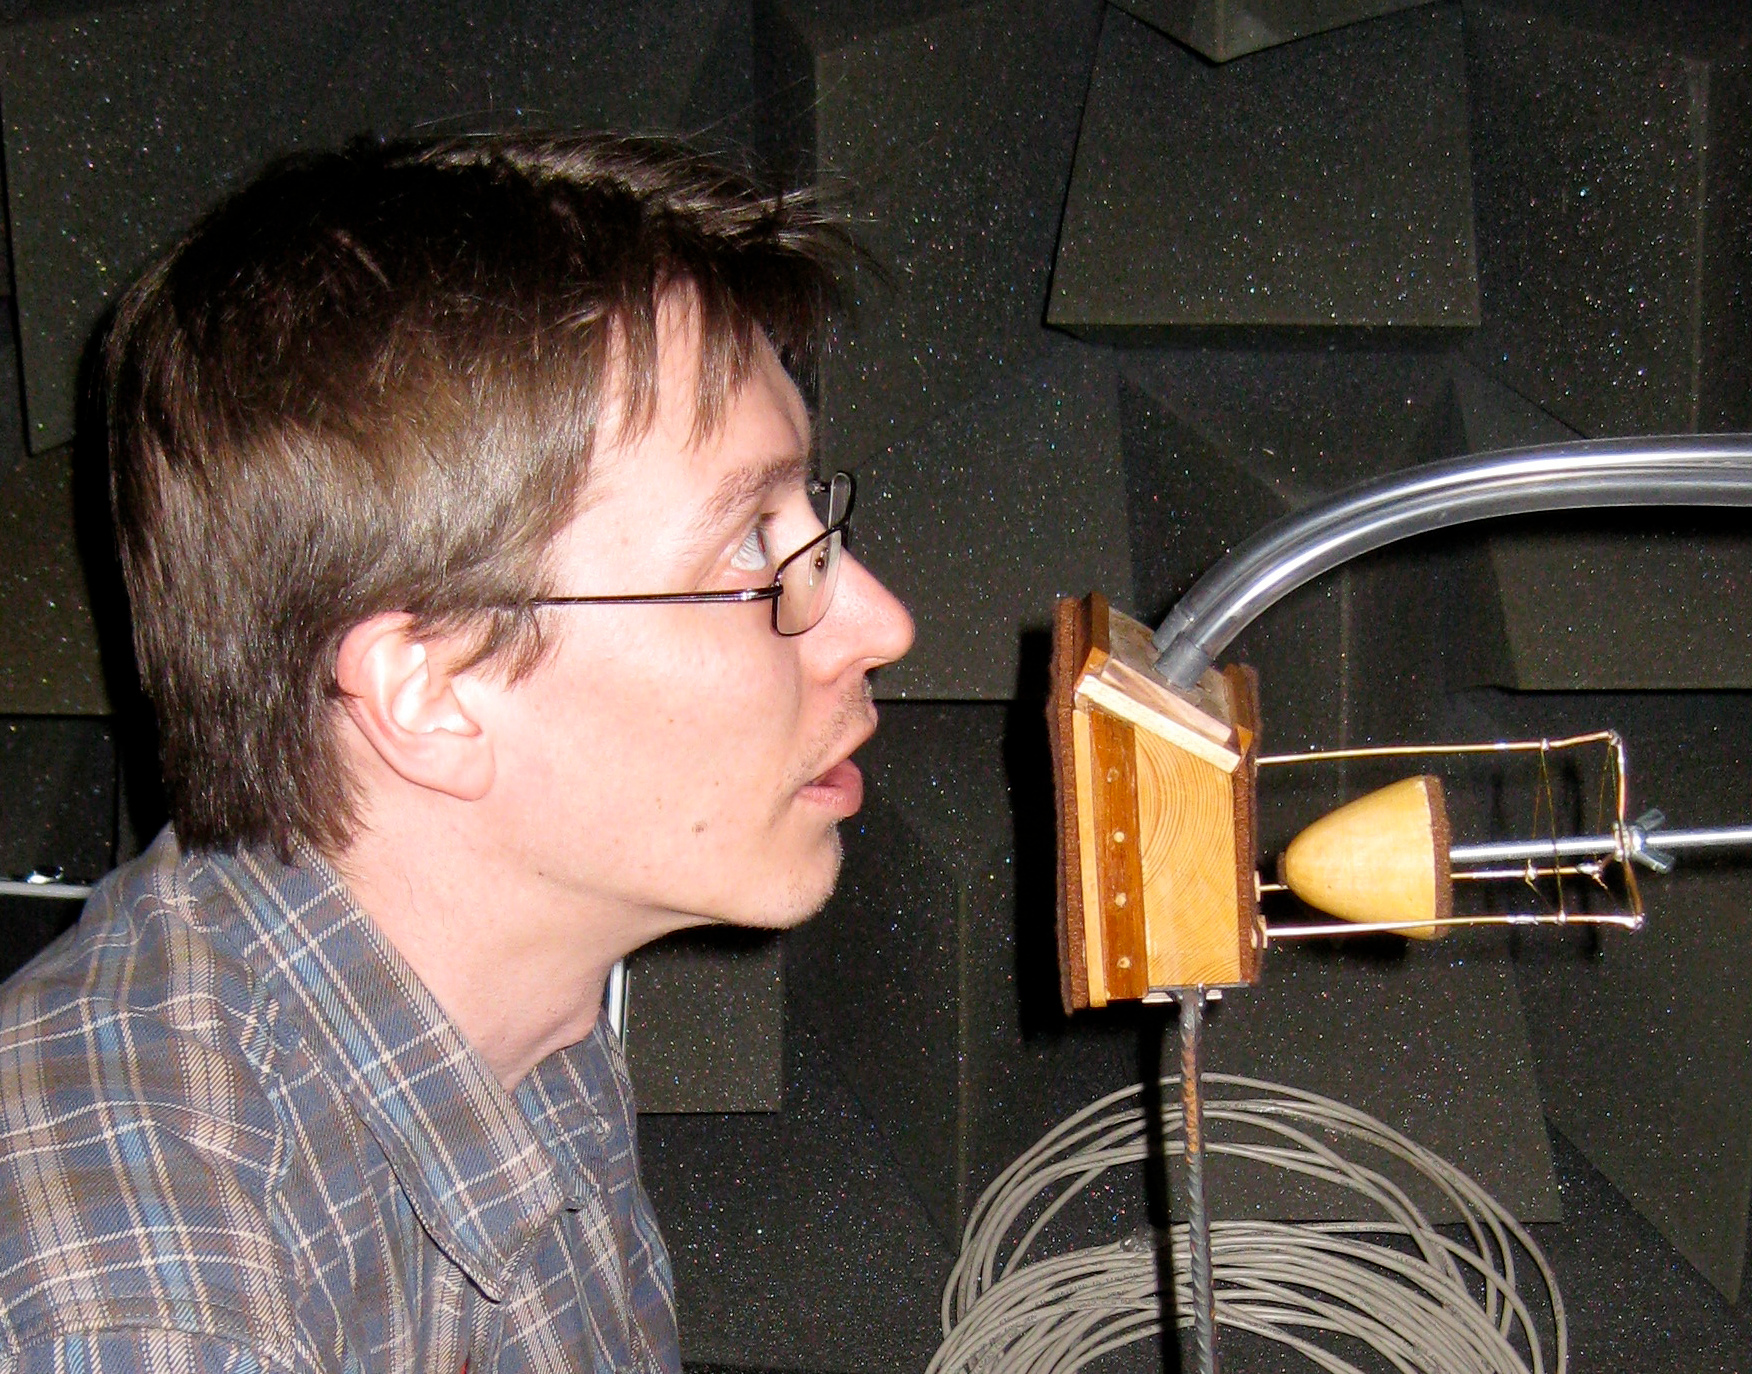
\includegraphics[height=3cm]{Pertti_sedan_letkuradio.jpg}
} 

\frame{\frametitle{Land acknowledgement}

% {\pigiarniq ᐊᒥᐢᑿᒌᐚᐢᑲᐦᐃᑲᐣ}

I live in amiskwacîwâskahikan / Edmonton. 

\note{
  \begin{itemize}
      \item I will keep it brief.
      \item Transition by noting that while my recent work has been in
    Edmonton, I am looking forward to bringing what I've learned here to
    Limerick and Ireland.    
  \end{itemize}
}
}



\frame{\frametitle{My three priorities}
\centering
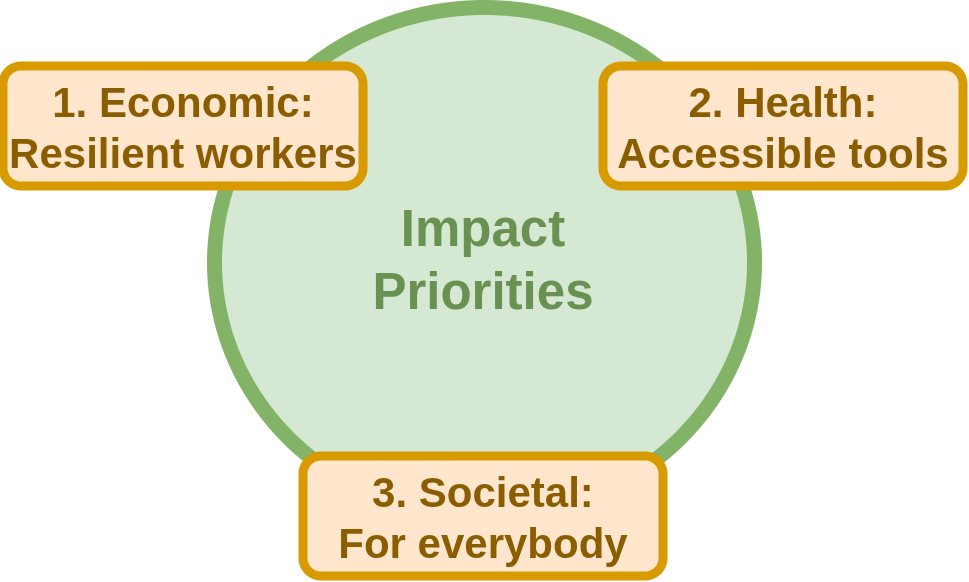
\includegraphics[height=.6\textheight]{infographic_big.png}

\note{  
\begin{enumerate}
  \item {\bf Economic Impact:} I train resilient and future-proofed workers.
  \item {\bf Health Impact:} I develop, teach, and advocate for accessible clinical tools.
  \item {\bf Societal Impact:} I work to ensure health systems and research
  serve the entire population.
\end{enumerate}
  \kommentti{how do these fit with the teaching philosphy and research impact?}
  \begin{itemize}
  \item Knowledge and skills throughout studies and life (teaching and research)
  \item Articulation (teaching and research)
  \item Community engagement and decolonisation (teaching and research)
  \end{itemize}
  }
}


\frame{\frametitle{Priority 1: Training resilient and future-proofed workers}
\begin{columns}
  \begin{column}{.8\textwidth}
    \begin{itemize}
      \item {\bf Foundational skills:} Finding, critiquing, and curating
      information in the age of AI.
      \item {\bf Intentional learning:} Integrating new methods into their
      professional practice.
      \item {\bf Learning environments:} I build the spaces and open source
      software
      \citep{Palo-CASTComputerAssisted-2024,PaloEtAl-PATKITPhoneticAnalysis-2026,PaloLaporte-SLURPYPythonVersion-2026}
      for students to learn in practice and think critically about tongue
      ultrasound \citep{Palo-MeasuringPrespeechArticulation-2019}, air flow
      \citep{PaloCowen-SimultaneousRecordingTongue-2017}, electroglottography
      \citep{WaaramaaEtAl-EmotionsFreelyVarying-2014}, etc.
      \item {\bf Cross-disciplinary teaching:} I provide joint courses with other
      programs (University of Helsinki 2011-2012) to teach students collaboration with 
      physicians, occupational therapists, physical therapists, engineers, etc.
    \end{itemize}    
  \end{column}
  \begin{column}{.18\textwidth}
    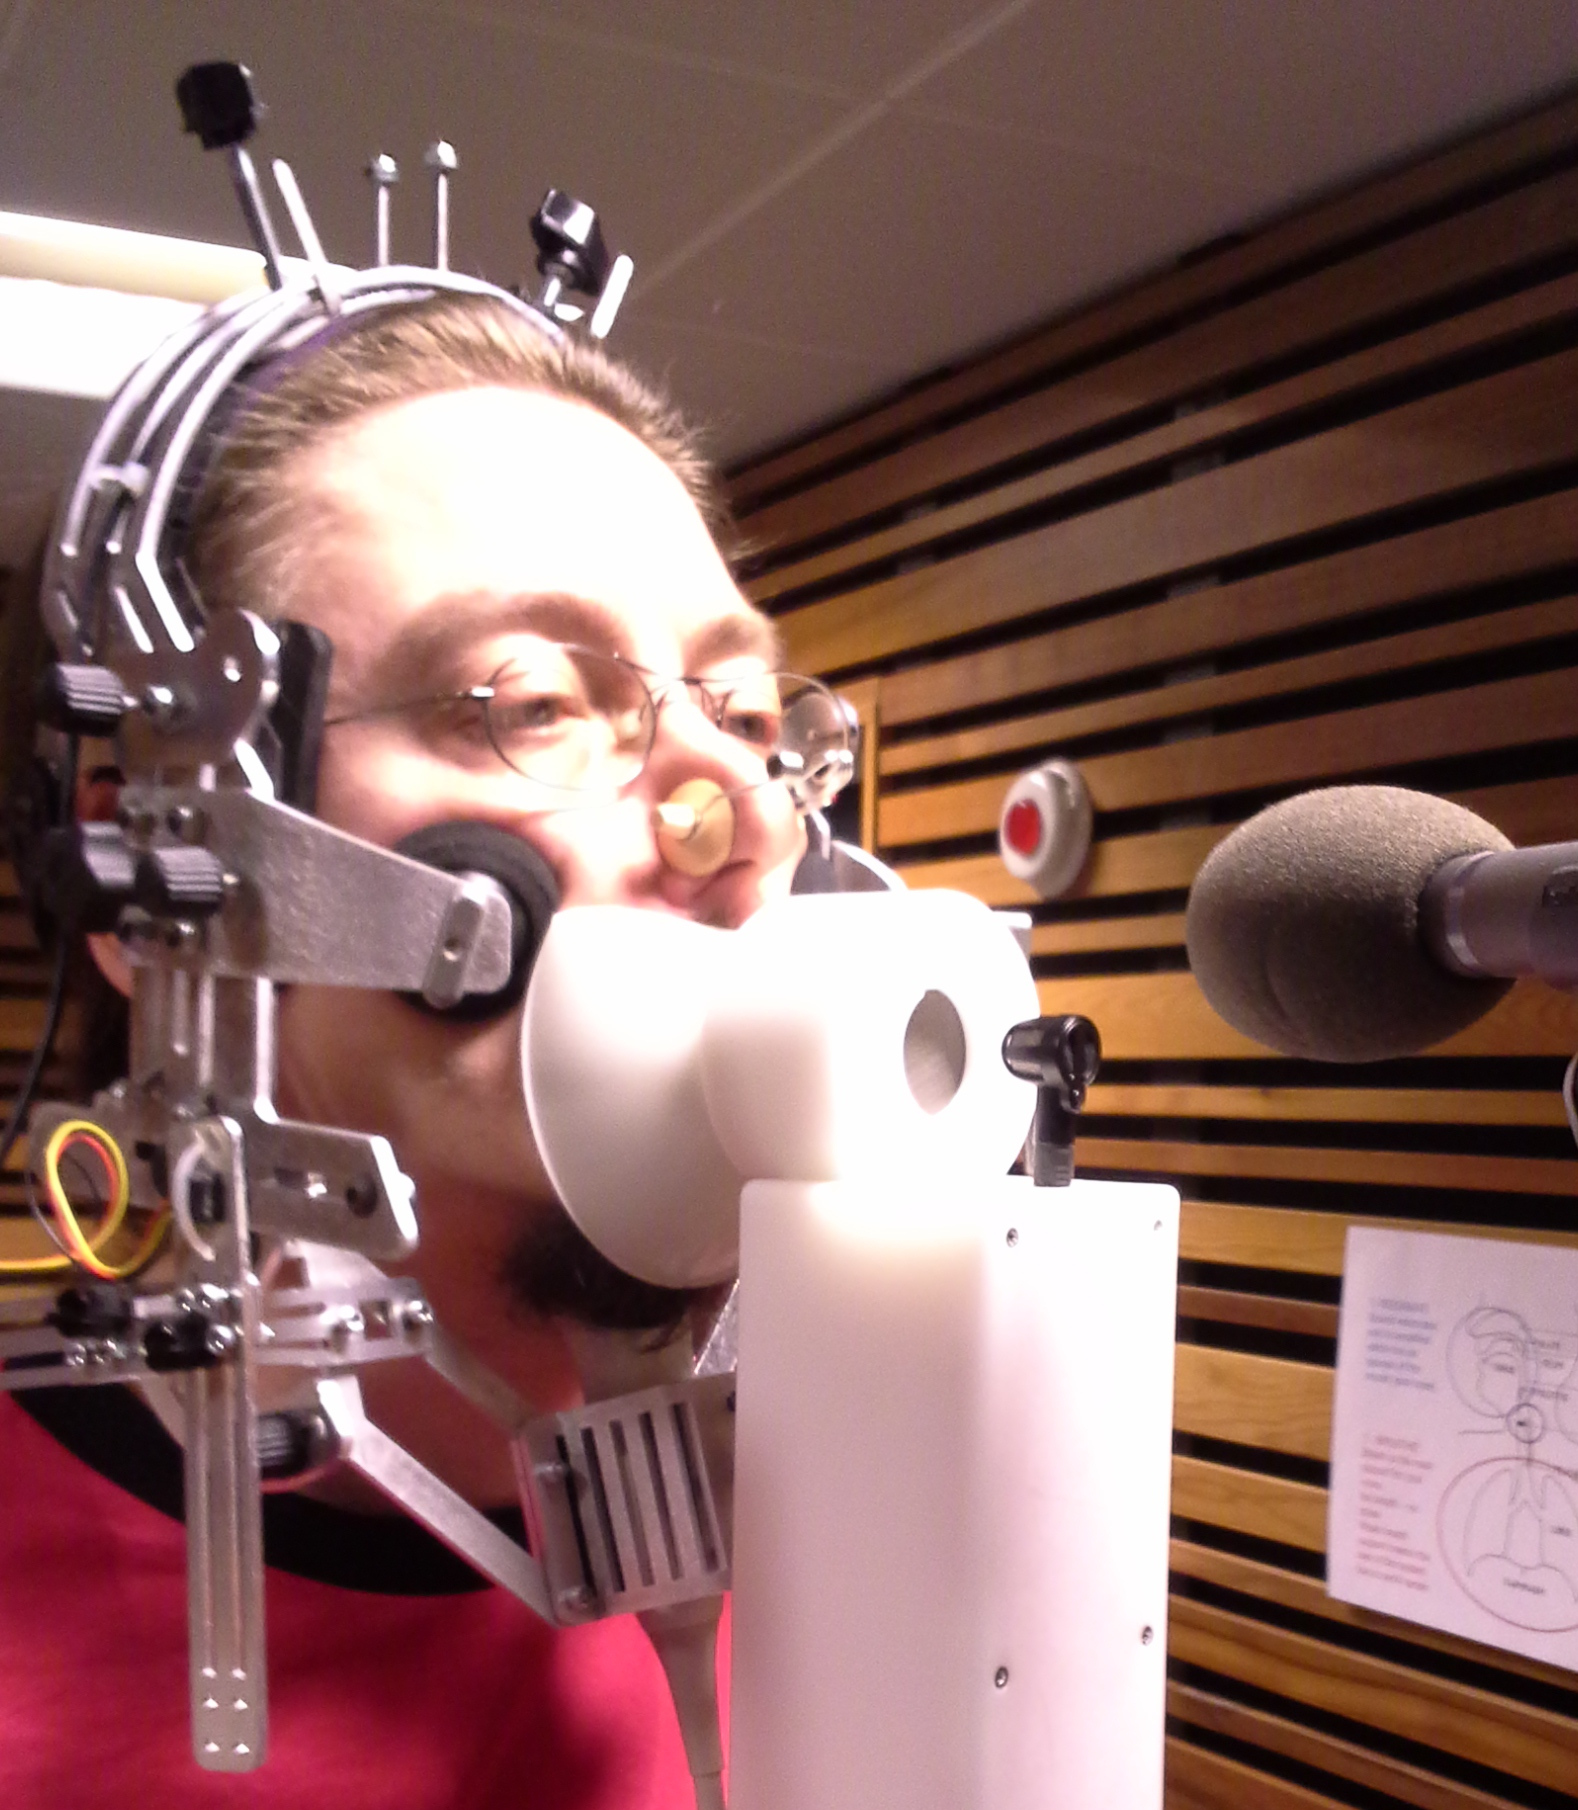
\includegraphics[width=\columnwidth]{ultra-eva.jpg}
    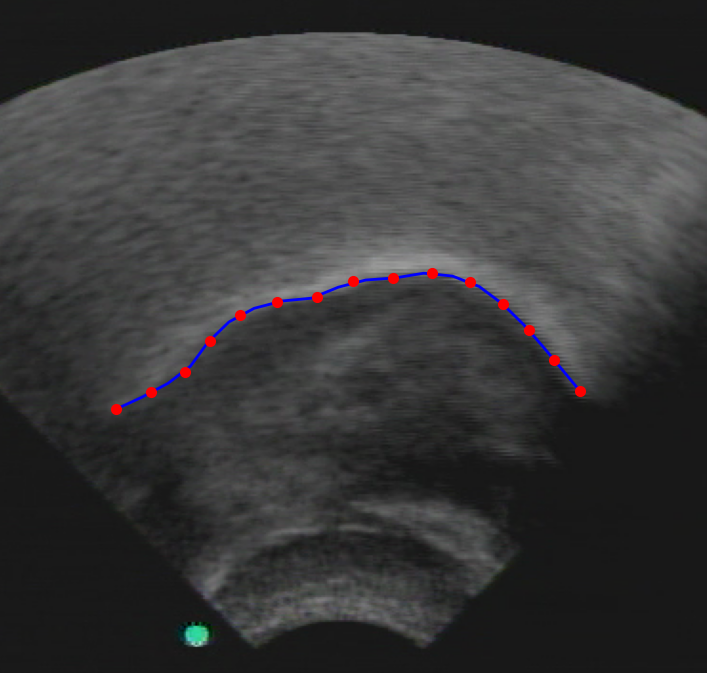
\includegraphics[width=\columnwidth]{slurp.png}
  \end{column}
\end{columns}

\note{  
  \kommentti{Employ some dry humour here. You might note that while instilling a
  love of learning is a noble academic pursuit, from a purely pragmatic impact
  perspective, teaching students "how to learn" ensures that the graduates UL
  produces don't become professionally obsolete the moment a new technology is
  introduced to the clinic.}
  \begin{itemize}
  \item Resilience is not just an attitude. It comes from having the skills to
  work with other professionals and with new tools and changing situations.
  \item example on learning with intention
  \item example on learning a new method and integrating it
  \end{itemize}
  }
}



\frame{\frametitle{Priority 2: Accessible clinical tools}
\begin{columns}
  \begin{column}{.8\textwidth}
    \begin{itemize}
    \item {\bf Articulatory methods:} Needed to understand speech production by
    linking neural processes and the produced acoustic speech.
    \item {\bf Ultrasound:} Relatively cheap, very portable, and intuitive for
    users who are knowledgeable in articulation and anatomy. 
      \begin{itemize}
      \item {\bf Speech pathologies:} I use ultrasound in studying stuttering,
      Parkinsons disease, and covert errors
      \citep{LloydEtAl-ImpactRealtimeArticulatory-2019}.
      \item {\bf Biofeedback:} Patients and clients quickly orient to their own
      articulation. 
    \end{itemize}
    \item {\bf Tool demonstrations:} 
      \begin{itemize}
      \item Ultrasound video of silent speech articulation in stuttering.
      \item Speech analysis with PATKIT \citep{PaloEtAl-PATKITPhoneticAnalysis-2026}.
      \end{itemize}
    \end{itemize}
  \end{column}
  \begin{column}{.18\textwidth}
    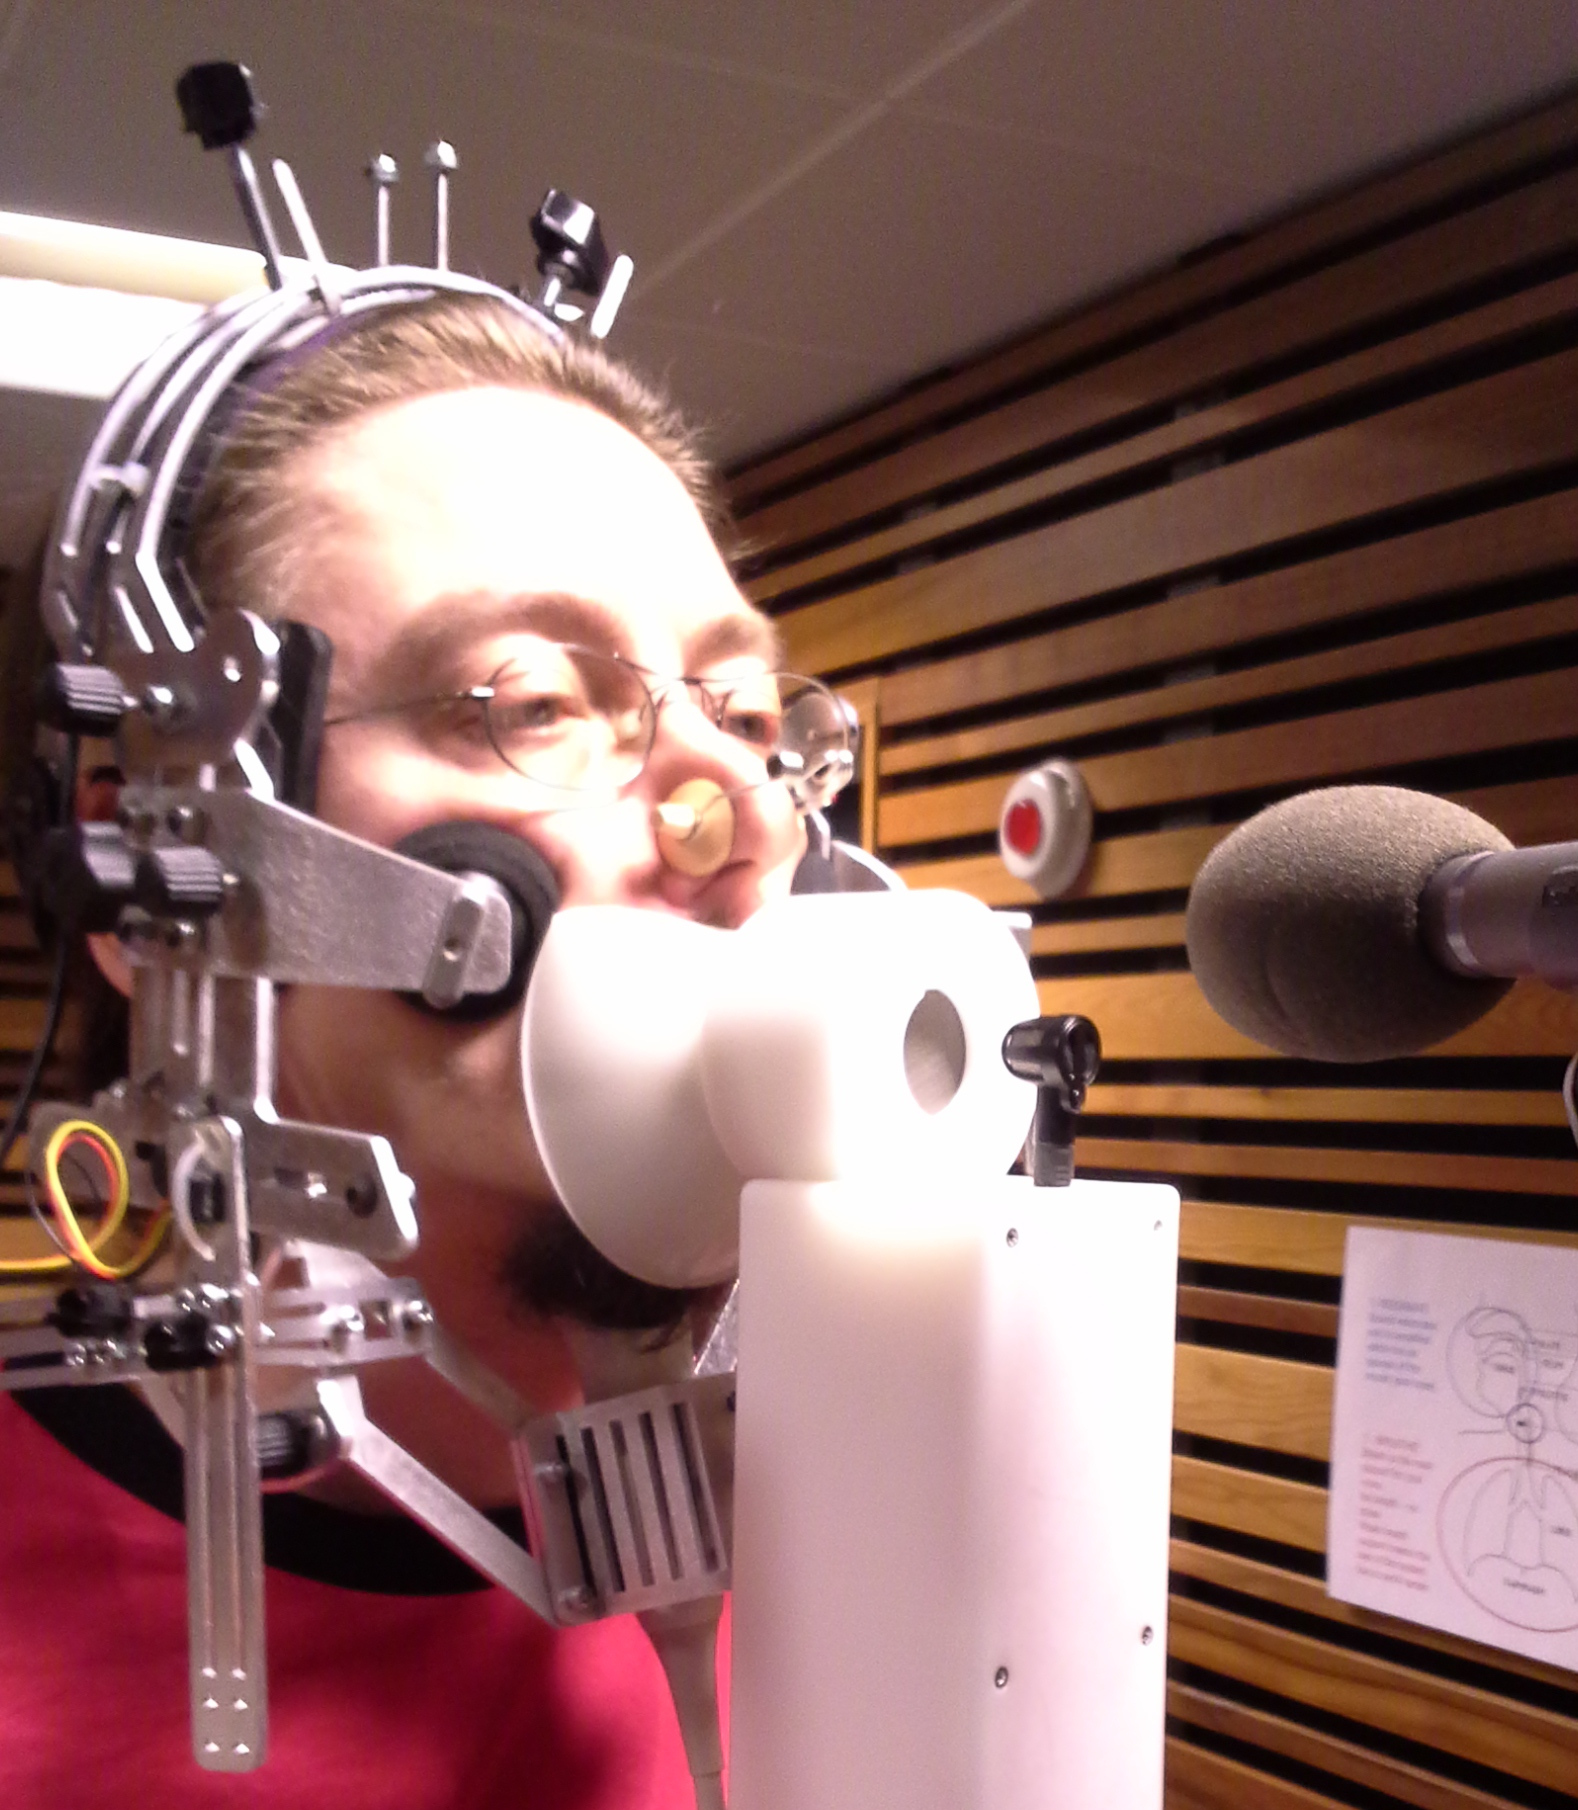
\includegraphics[width=\columnwidth]{ultra-eva.jpg}
    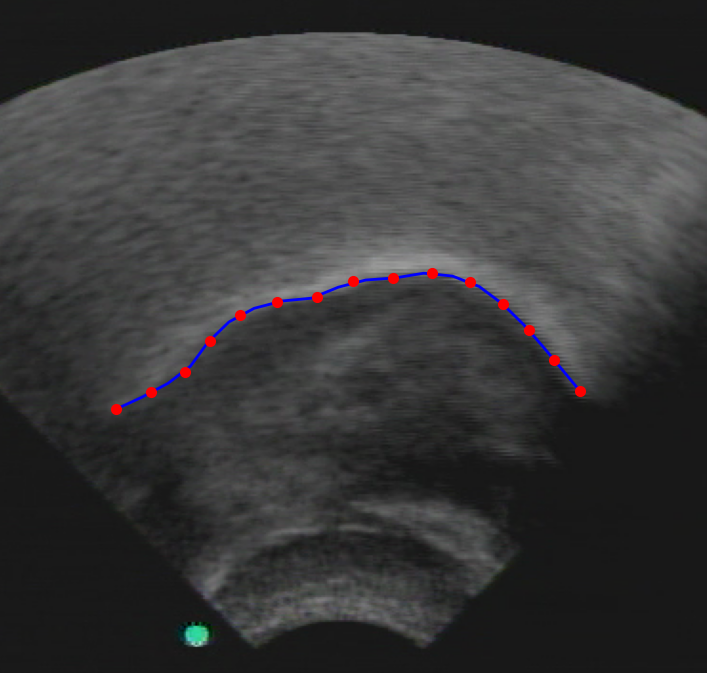
\includegraphics[width=\columnwidth]{slurp.png}
  \end{column}
\end{columns}

\note{  
  \kommentti{Make the clinical translation the star of the slide. In impact
  terms, means ultrasound can be deployed in standard community clinics -- or
  even a mobile clinic, democratizing access to biofeedback and other clinical
  applications, rather than keeping it locked behind the doors of a research
  hospital.}
  \begin{itemize}
  \item "in research, teaching and clinical work" Articulation provides a
  deeper understanding of speech production: It links neural processes and the produced speech.
  \item Cost effectiveness and portability make it more accessible as
  evaluations can be done in local clinics or even in mobile clinics.
  \item 
  \end{itemize}
  }
}


\frame{\frametitle{Ultrasound stuttering example}

  \kommentti{Link to youtube video}
}

\frame{\frametitle{PATKIT example}
  \centering
  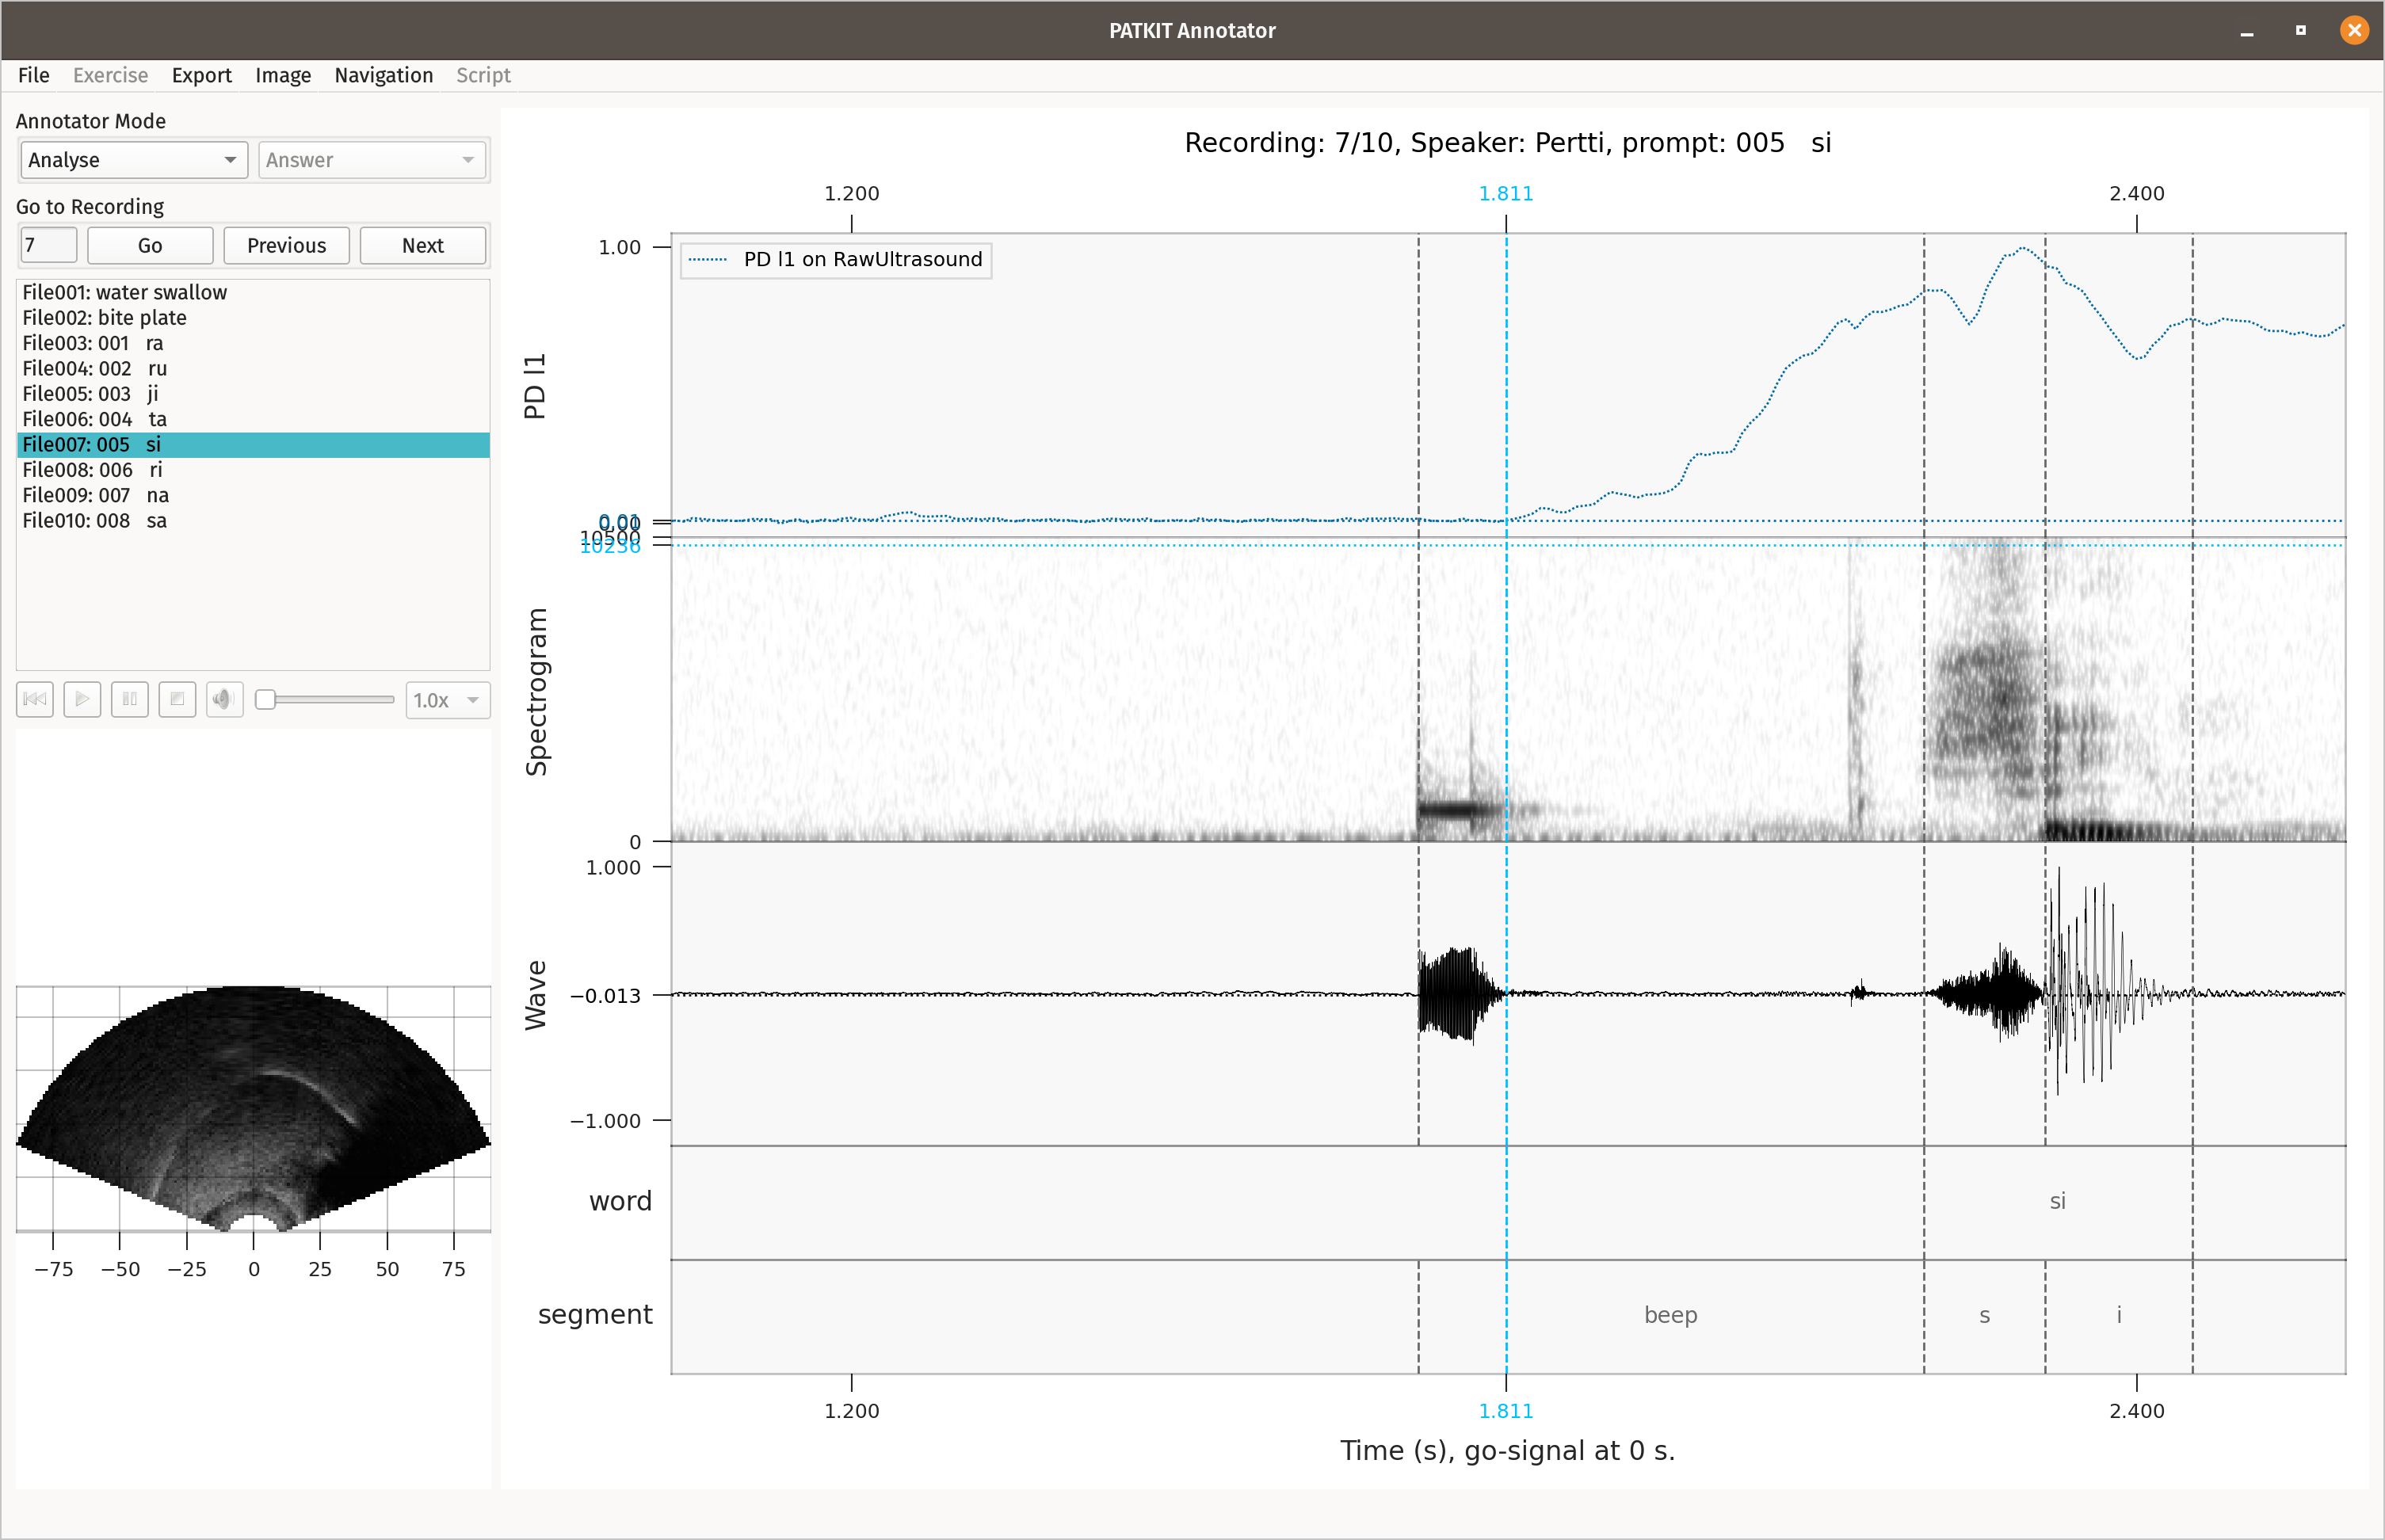
\includegraphics[width=.8\textwidth]{PATKIT-zoomed-example.png}
\note{   
  The Transition: "I am an experimental phonetician, which means I could very
  happily spend the remainder of the day just discussing PATKIT and the
  articulatory mechanics of the tongue in that video. But if the baseline
  data we use comes from a narrow, privileged demographic, our research and
  clinical outcomes will be fundamentally flawed. Therefore, my third
  priority is..." 
  } 
}



\frame{\frametitle{Priority 3: Serving the entire population}
\begin{columns}
  \begin{column}{.8\textwidth}
    \begin{itemize}
    \item {\bf  Health systems and research for all:} Decolonisation and social
    justice are tools for ensuring our work is for all of humanity and not just a
    fraction. % \citep{LonnqvistEtAl-HowYoungAdults-2017}. 
    \item {\bf Outreach experience:} I regularly contribute to a role-playing
    convention in Finland on, e.g., responsible
    use of existing languages in fictional settings (Ropecons 2022-2025). 
    \item {\bf Connection skills:} For the last two years I have been building
    relationships with and learning relationship building from Indigenous
    communities in and around Edmonton.
    \item {\bf Community connection building:} My skills will be useful in
    working with the The Gaeltacht, the Traveller community and migrant
    populations. 
    \end{itemize}
  \end{column}
  \begin{column}{.18\textwidth}
    
\includegraphics[width=\columnwidth]{ropecon_cropped.jpg}
    
\includegraphics[width=\columnwidth]{SaddleLakeCreeNation.png}
  \end{column}
\end{columns}

  \note{
    
    \begin{itemize}
      \item The mention of the Finnish role-playing convention is meant as a
    slightly quirky detail to make me less two dimensional. I will deliver it
    entirely deadpan.  Then, pivot strictly to the core message:
    "Representative research is not just a moral imperative; it is a
    methodological requirement to ensure that the health systems we design
    actually work for the entire population."
    \item Mention that all of the engagement I do is with active collaborators:
    we all learn in the process and we all teach.
  \end{itemize} 
  } 
}


\frame{\frametitle{First concrete steps on my impact priorities}

\begin{columns}
  \begin{column}{.24\textwidth}
    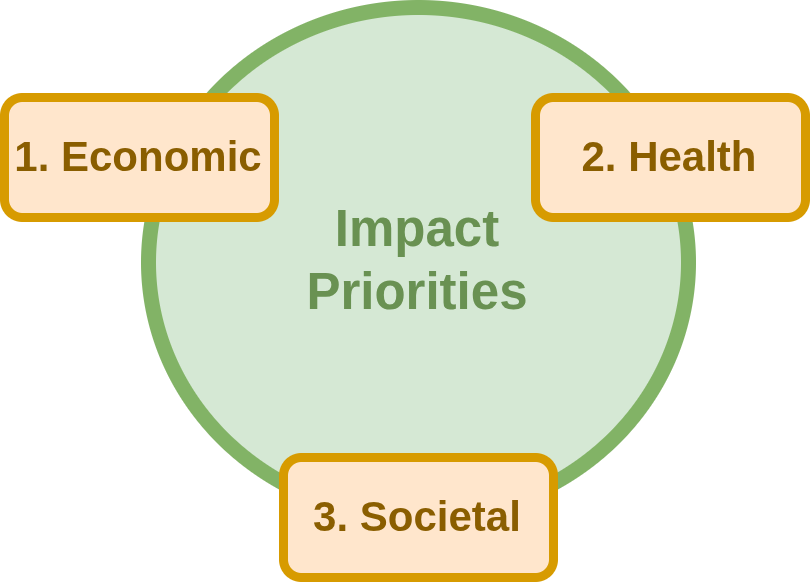
\includegraphics[width=\columnwidth]{infographic.png}
  \end{column}
  \begin{column}{.75\textwidth}
    \begin{enumerate}
      \item {\bf Economic:} I will set up a world class teaching
      laboratory at University of Limerick. With my experience (University of
      Helsinki 2020, University of Alberta 2024-2026), I can fit the lab in
      limited or temporary spaces.
      \item {\bf Health:} I am preparing an international project to study
      articulatory stability in Parkinsons with ultrasound. This will be a major EU
      grant with collaborators from Canada and Finland with methods I have
      developed over the past decade
      \citep{Palo-MeasuringPrespeechArticulation-2019,PaloEtAl-MagnitudeUltrasoundProbe-2025,
      PaloEtAl-PATKITPhoneticAnalysis-2026}.  
      \item {\bf Societal:} Inspired by
      \cite{Ladefoged-PhoneticDataAnalysis-2003} and
      \cite{RebernikEtAl-SPRAAKLABMobileLaboratory-2025} I will bring speech
      research and therapy to the whole population by building a mobile lab/clinic
      in a van as a major grant funded project.
    \end{enumerate}
  \end{column}
\end{columns}

  \note{
    
    \begin{itemize}
    \item The mention of the Finnish role-playing convention is meant as a
    slightly quirky detail to make me less two dimensional. I will deliver it
    entirely deadpan. Then, pivot strictly to the core message:
    "Representative research is not just a moral imperative; it is a
    methodological requirement to ensure that the health systems we design
    actually work for the entire population."
    \item Mention that all of the engagement I do is with active collaborators:
    we all learn in the process and we all teach.
  \end{itemize} 
  } 
}


\frame{
  \centering
  {
    \bf \Large 
    \usebeamercolor[fg]{title}
    Thank you!\\
    \vfill
    Go raibh maith agaibh!
    \vfill
%    \includegraphics[height=1.5cm]{figures/aalto_logo} 
  }
}

\frame{\frametitle{References}

\tiny
\bibliographystyle{apalike}
\bibliography{science_combined}

}

\end{document}


\begin{frame}
 \begin{itemize}
 \item<1-> Eggs
 \item<2-> Plants
   \note[item]<2>{Tell joke about plants.}
   \note[item]<2>{Make it short.}
 \item<3-> Animals
 \end{itemize}
\end{frame}



% \frame{\frametitle{Knowledge and skills throughout studies and life: Foundational knowledge}
%   \begin{itemize}
%   \item Instrumentation: Sound, Articulation, flow, etc
%   \item Acoustic phonetics
%   \item Articulatory phonetics ()
%   \item Perceptual phonetics (\kommentti{what actually matters in perception})
%   \item Anatomy and physiology (from a functional point of view, how used in
%   speech, how used in other activities)
%   \item Neurolinguistics (Levelt, DIVA and other theories and models)
%   \end{itemize}

%   The idea is to build a solid foundation for the students so that they'll find
%   it easy to add new, more complex concepts, find connections between what they
%   have and are learning, and to pose questions to their own understanding and
%   to their instructors and materials.

% }


% \frame{\frametitle{Knowledge and skills throughout studies and life: Life long learning}
%   \begin{itemize}
%   \item Students should not come to university to do a degree and be done with
%   learning. In fact, their attitude from the beginning should be that they are
%   learning to learn, so that they can keep on doing so for the rest of their
%   lives.
%   \item From the get go I want to teach students how to find and evaluate
%   knowledge themselves. 
%   \item Seminar presentations and thesis work bring depth to learning and
%   enhance information finding and critiquing skills.
%   \item My goal is that after graduation the new SLTs will be motivated to
%   continue to read scientific articles and to both update their knowledge and
%   keep an active relationship with researchers. This will not be a one way
%   street of researchers only providing information and ideas, but rather an
%   on-going discussion and sharing of information of ideas between colleagues
%   some of whom do research and some clinical work.
%   \end{itemize}
% }